\subsection{Description}
The Poisson distribution expresses the probability of a given number of events occurring in a fixed interval of time or space if these events occur with a known constant mean rate and independently of the time since the last event. The Poisson distribution can also be used for the number of events in other specified intervals such as distance, area or volume.

For instance, an individual keeping track of the amount of mail they receive each day may notice that they receive an average number of 4 letters per day. If receiving any particular piece of mail does not affect the arrival times of future pieces of mail, i.e., if pieces of mail from a wide range of sources arrive independently of one another, then a reasonable assumption is that the number of pieces of mail received in a day obeys a Poisson distribution. Other examples that may follow a Poisson distribution include the number of phone calls received by a call center per hour, the number of decay events per second from a radioactive source, the number of visits to a website and the number of typographical errors per page in a book.

The Poisson distribution is an appropriate model if the following assumptions are true:

\begin{itemize}
	\item k is the number of times an event occurs in an interval and k can take values 0, 1, 2, ....
	\item The occurrence of one event does not affect the probability that a second event will occur. That is, events occur independently.
	\item The average rate at which events occur is constant.
	\item Two events cannot occur at exactly the same instant; instead, at each very small sub-interval exactly one event either occurs or does not occur.
\end{itemize}


\subsubsection{Probability mass function}
Let $X$ denote the number of events in a unit interval of time or in a unit distance.Then, $X$ is called the Poisson random variable with mean number of events $\lambda$ in a unit interval of time. The probability mass function of a Poisson distribution with mean $\lambda$ is given by
\[
 	f(k \mid \lambda) = P(X = k \mid \lambda) = \frac{e^{-\lambda} \lambda^k}{k!}, \ k = 0, 1, 2, \ldots
\]

The Poisson probability mass function is right-skewed, and the degree of skewness decreases as $\lambda$ increases.

\begin{figure}[H]
	\centering
	\begin{subfigure}[b]{0.45\textwidth}
		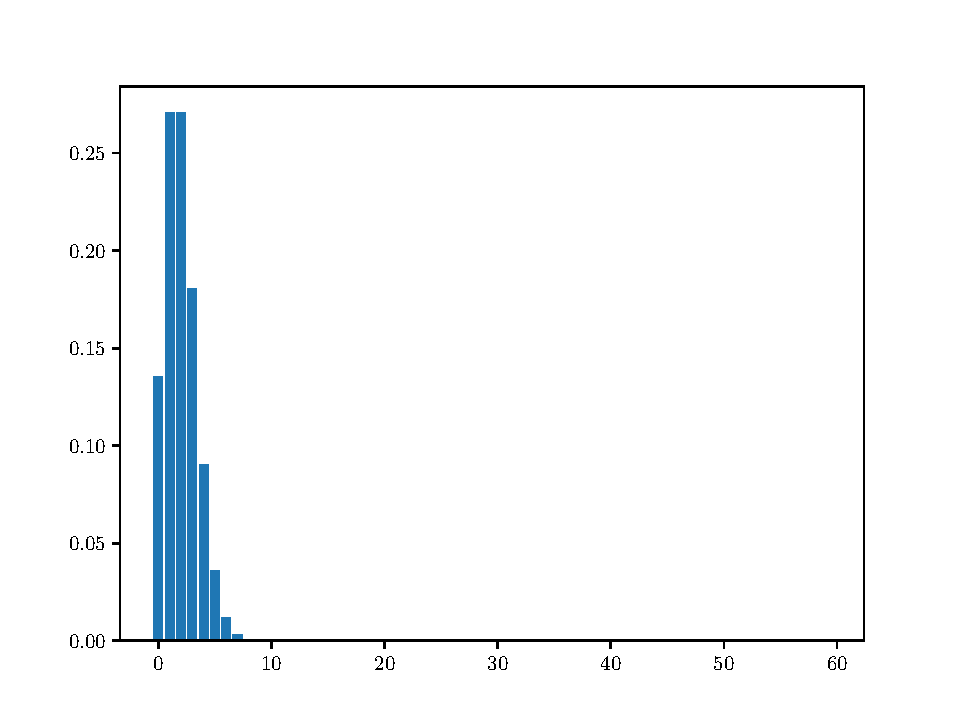
\includegraphics[width=\textwidth]{discrete/poisson/pmf_2.pdf}
		\caption{$\lambda = 2$}
		\label{fig:P2}
	\end{subfigure}
	\begin{subfigure}[b]{0.45\textwidth}
	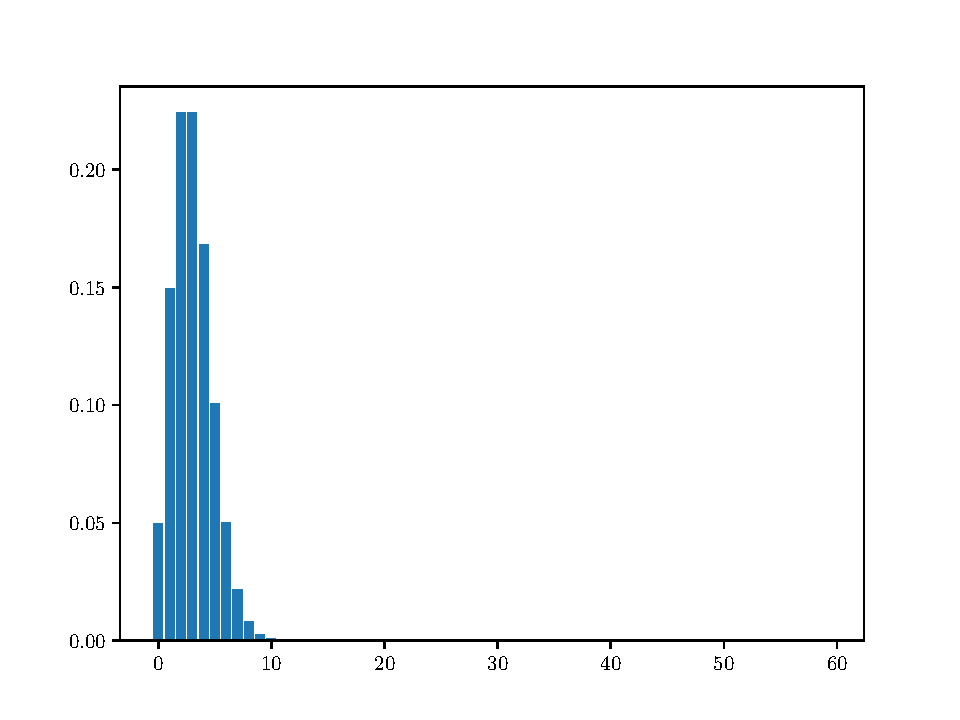
\includegraphics[width=\textwidth]{discrete/poisson/pmf_3.pdf}
	\caption{$\lambda = 3$}
	\label{fig:P3}
	\end{subfigure}
	\begin{subfigure}[b]{0.45\textwidth}
		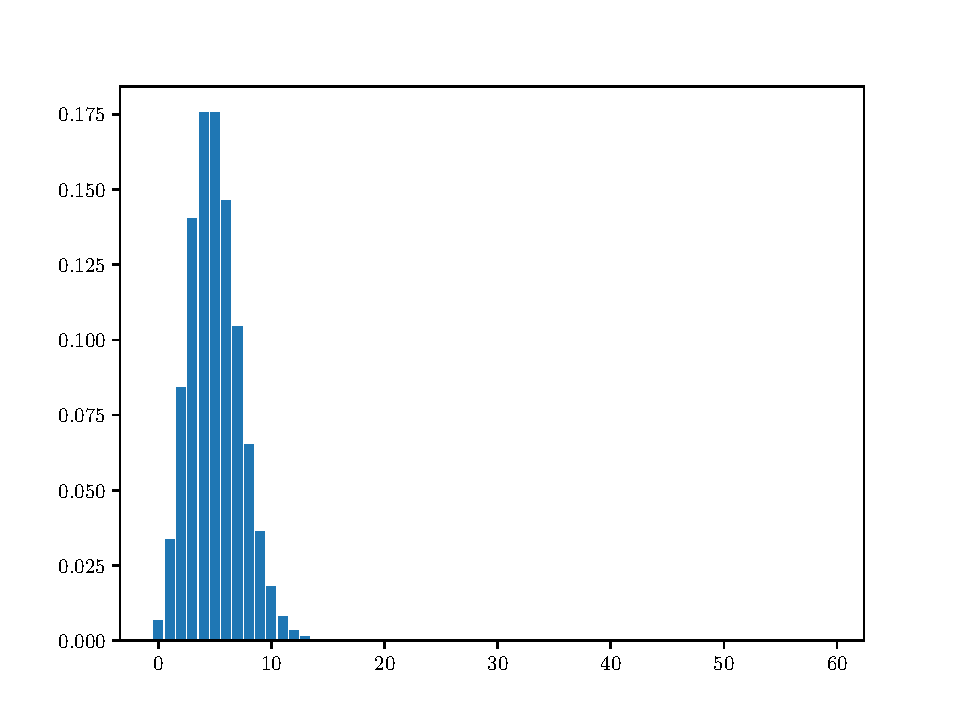
\includegraphics[width=\textwidth]{discrete/poisson/pmf_5.pdf}
		\caption{$\lambda = 5$}
		\label{fig:P5}
	\end{subfigure}
	\begin{subfigure}[b]{0.45\textwidth}
		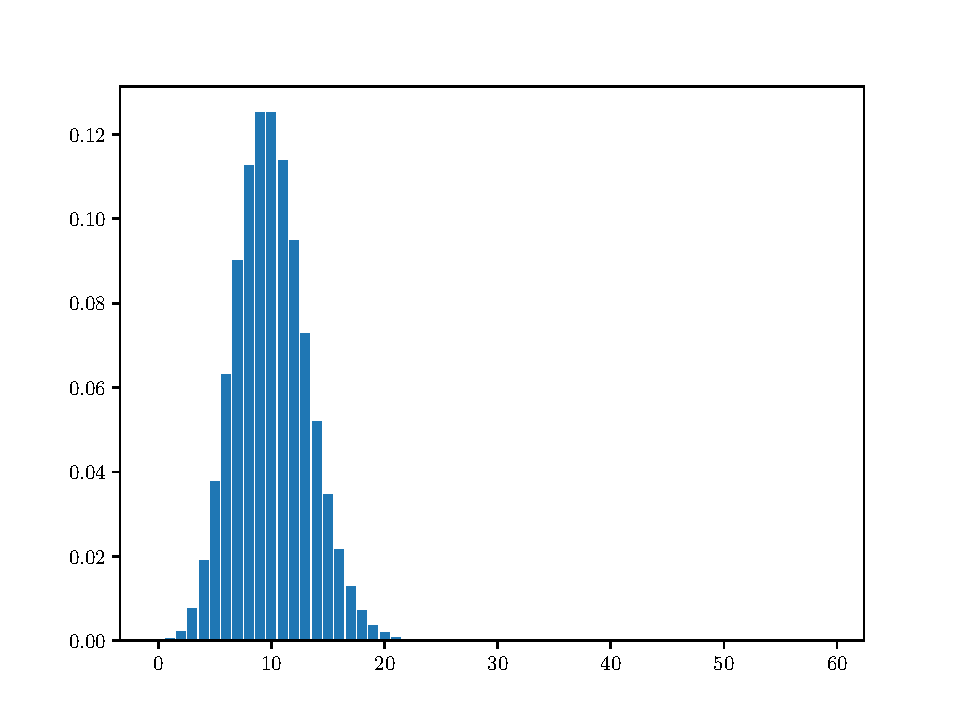
\includegraphics[width=\textwidth]{discrete/poisson/pmf_10.pdf}
		\caption{$\lambda = 10$}
		\label{fig:P10}
	\end{subfigure}
	\begin{subfigure}[b]{0.45\textwidth}
		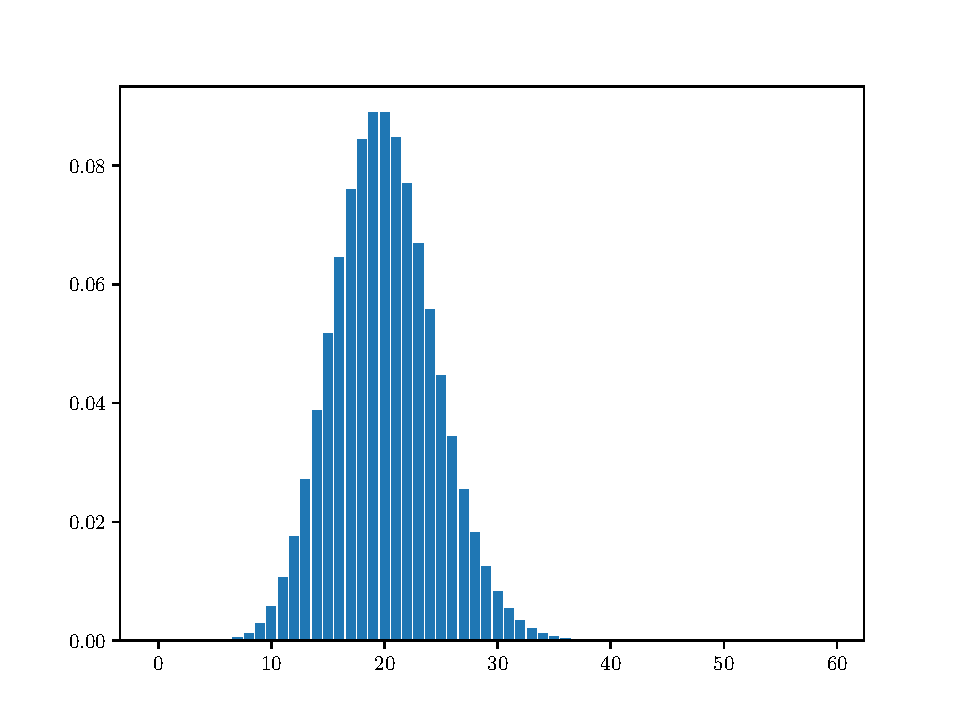
\includegraphics[width=\textwidth]{discrete/poisson/pmf_20.pdf}
		\caption{$\lambda = 20$}
		\label{fig:P20}
	\end{subfigure}
	\begin{subfigure}[b]{0.45\textwidth}
		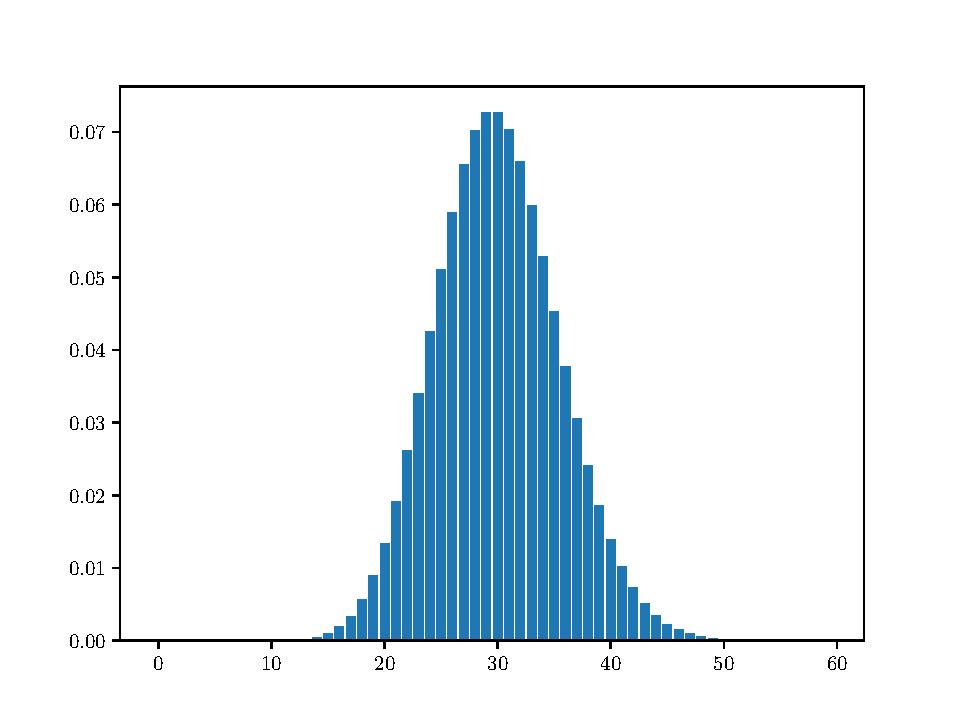
\includegraphics[width=\textwidth]{discrete/poisson/pmf_30.pdf}
		\caption{$\lambda = 30$}
		\label{fig:P30}
	\end{subfigure}
	\caption{Poisson distribution}\label{fig:poisson}
\end{figure}

\begin{figure}[H]
	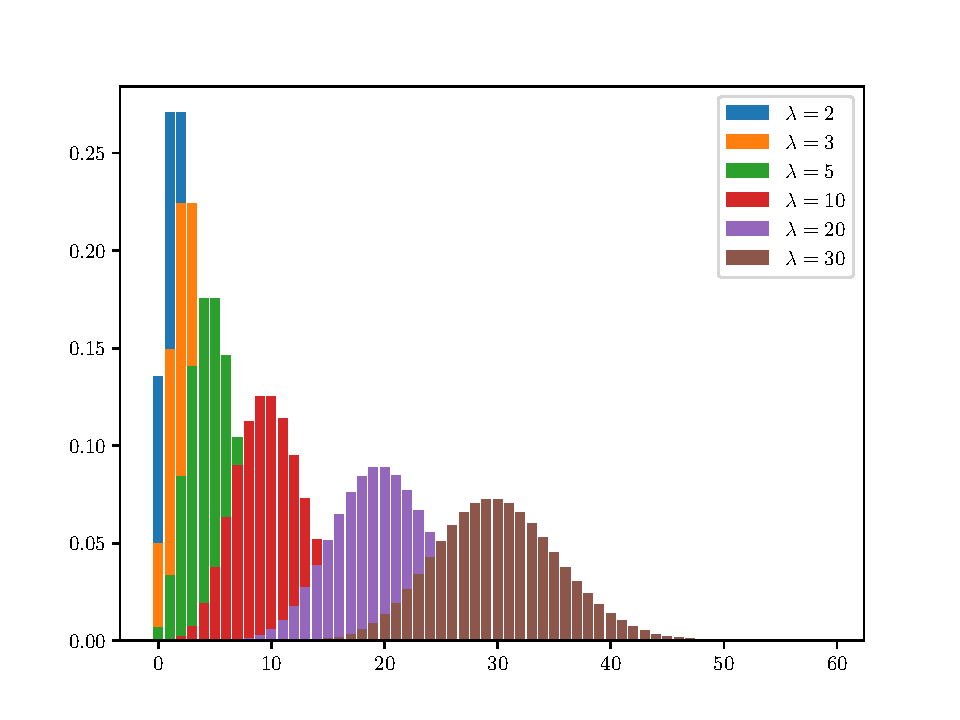
\includegraphics[width=\textwidth]{discrete/poisson/pmf_all.pdf}
	\caption{$f(k \mid \lambda) = P(X = k \mid \lambda) = \frac{e^{-\lambda} \lambda^k}{k!}, \ k = 0, 1, 2, \ldots$}
\end{figure}

\subsubsection{Cumulative distribution function}
\[
	F(k \mid \lambda) = P(X = k \leq \lambda) = \sum_{i = 0}^{k} \frac{e^{-\lambda} \lambda^i}{i!}, \ k = 0, 1, 2, \ldots
\]

The Poisson distribution can also be developed as a limiting distribution of the binomial, in which $n \rightarrow \infty$ and $p \rightarrow 0$ so that $np$ remains a constant. In other words, for large $n$ and small $p$, the binomial distribution can be approximated by the Poisson distribution with mean $\lambda = np$.

If the sample was drawn without replacement from a small finite population, the hypergeometric distribution should be used instead of the binomial.

\subsection{Moments}

\begin{tabularx}{\textwidth}{s X}
	\hline
	Mean & $\lambda$ \\\hline
	Variance & $\lambda$\\\hline
\end{tabularx}
